\documentclass[letterpaper]{exam}

\setlength\parindent{0pt}
\usepackage[utf8]{inputenc}
\usepackage[T1]{fontenc}
\usepackage{textcomp}
\usepackage{amsmath, amssymb}
\usepackage{graphicx}
\graphicspath{ {./images/} }
\title{Study Guide: Unit 1}
\author{Svadrut Kukunooru}
\date{\today}

\begin{document}
\begin{titlepage}
    \maketitle
\end{titlepage}
\begin{figure}[t]
    \centering
    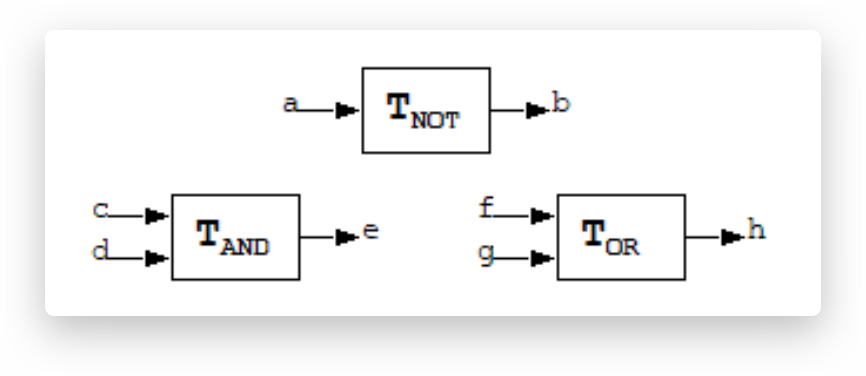
\includegraphics[width=0.5\textwidth]{turing1}
    \caption{Turing Machines}
\end{figure}
   \begin{questions}
       \question You are given the following three simple Turing Machines that implement the logic operations NOT, AND, and OR, and their connections are labeled with the letters a through h. Refer to Figure 1. Connect these simple machines to form the logical function exactly as shown below (no simplifying the function): ((NOT 1) AND 2) OR 3
       \begin{checkboxes}
        \choice input 1 connects to c 
        \choice e connects to g
        \choice input 1 connects to a
        \choice input 3 connects to c 
        \choice h connects to a
        \choice input 2 connects to d 
        \choice b connects to c
       \end{checkboxes}
              \question Assume each choice below shows the addition of two 6-bit fixed-point binary integers. Mark every choice that results in overflow. 
              \begin{checkboxes}
                \choice 0111.10 + 0000.11
                \choice 1010.10 + 1101.01 
                \choice 0011.01 + 0100.10
                \choice 1110.10 + 0001.10
                \choice 1010.10 + 1100.00
              \end{checkboxes}
              \question Assume each integer shown below is in base 10. Use 7 bits to show each integer in the representation listed. If it is \textit{not} possible to show the integer in the representation listed, answer "xxxxxxx".            \begin{parts}
                \part 0 in signed magnitude.
                
                \part -22 in 2's complement. 
                
                \part 37 in 2's complement. 
                
                \part -44 in unsigned. 
       \end{parts}
       \question Convert $1.75_{10}$ to its equivalent in IEEE 754 32-bit floating point representation. Be careful when entering your 32-bit answer. 
       \question Assume each choice below shows the addition of two 4-bit 2's complement binary integers. Mark every choice that results in overflow. FYI: Be certain; Canvas deducts points for incorrect choices. 
       \begin{checkboxes}
            
            \choice 1011 + 1100

            \choice 0111+0010

            \choice 1011+1010

            \choice 1110 + 1010
            
            \choice 0110 + 1010 
            
            
       \end{checkboxes}
       \question Consider the following 10-bit fixed-point binary value 0111011.011; what is its value in bae 10 with three digits of precision after the decimal point?
       \question Assume that there are 220 books in a library. If every book is to be assigned a unique bit pattern, what is the minimum number of bits required to do this? Additionally, what are the number of books that can be added to the library without requiring additional bits for each book's unique bit pattern? 
       
       \question Determine if each of the following pairs of logical expressions are equivalent. HINT: For each pair, use a truth table to show that for all combinations of inputs (i.e., for X only 0,1; for X and Y 00,01,10,11) both expressions produce the same results. 
       \begin{parts}
            \part NOT(NOT(NOT(X))) = NOT(X) ARE equivalent
            
            \part NOT(X OR Y) = NOT(X) AND NOT(Y) ARE equivalent
        \end{parts}
        \question Assume each value below shows an integer in 2's complement representation in 2,4,8 and 16 bits length. Convert each binary number to decimal. 
        \begin{parts}
            \part 11
            \part 1010 
            \part 10100111 
            \part 1101010011011001
        \end{parts}
        \question Convert $61543_{10}$ to its equivalent in unsigned integer format shown in hex(e.g., A27E) rather than binary. 
        \question You are given the following partial ASCII table of characters. (Just look up a table online, you're allowed to for this one). Which one of the following is NOT the correct 8 bit ASCII representation of the 3 character emoji? 
        \begin{checkboxes}
            \choice >:P is 00111110 00111010 01110000
            \choice :-( is 00111010 00101101 00101000
            \choice :\^) is 00111010 01011110 00101001
            \choice ;-] is 00111011 00101101 01011101
        \end{checkboxes}
        \question Which one of the logical calculations below takes 8-bit binary input X and clears to 0 its bits at odd positions leaving its bits at even positions unchanged, Recall, the left most bit is at position 7, which is an odd bit, and the rightmost bit iis at position 0, which is an even bit. 
        \begin{checkboxes}
           \choice X AND 01010101
           \choice X OR 01010101
           \choice X OR 10101010
           \choice X AND 10101010
        \end{checkboxes}
       \question Let X = 010101, Y = 001100 and Z = 101010. What is the result of (X OR (NOT Y)) AND Z? 
       \question Consider the following IEEE 754 32-bit floating point value 
       \[
       01001111\ 01001000\ 00000000\ 00000000
       .\] 
       Is its sign positive or negative? \\
       What is its exponent's value in base 10?\\ Enter the fraction part's value in base 10 in the format 0.XXXX where X is a digit. 
       \question Name a task you enjoy doing. Describe several high-level steps to complete that task. Next, take ach of these steps and break them down into detailed steps.

   \end{questions}
\end{document}
